\documentclass{apuntes}
\usepackage{anysize} 
\usepackage{dsfont}
\usepackage{amssymb}
\usepackage{textcomp}
\usepackage{plain}

%opening
\title{Estructuras algebraicas}
\author{Pedro Valero Mejía - Guillermo Ruiz Álvarez}
\date{13 / 14 C1}

\newenvironment{notacion}[1][Notación:]{\begin{trivlist}
\item[\hskip \labelsep {\bfseries #1}]}{\end{trivlist}}

\begin{document}

\pagestyle{plain}
\maketitle
\tableofcontents
\newpage

\section{Grupos}
 
 \subsection{Conceptos generales}
 Por definición, sea X un conjunto no vacío, podemos construir el conjunto de pares ordenados $X\ast X=\{(x,y)\tq x,y\in X\}$
 
 Vamos a fijar un conjunto $X\neq \emptyset$  y una función $\appl{\varphi}{X\ast X}{X}$ que a cada par $(x,y)$ le 
 asocia un elemento $\varphi(x,y) \in X$ que expresamos como $x\ast y$, siendo '$\ast$' cualquier operación.
 
 \begin{defn}[Subconjunto\IS cerrado]
  Sea S un subconjunto no vacío de G, diremos que S es cerrado por $\varphi$  si la combinación por $\varphi$  de dos elementos de
  S da otro elemento del mismo.
 \end{defn}
 
 Dados $x,y,z \in X$ puede ser interesante el resultado $x\ast y\ast z$ pero, por definición, esto no tiene sentido. Sin embargo, si tendrían 
 sentido $(x\ast y)\ast z$ ó $x\ast (y\ast z)$. Estas operaciones podrían tener, o no, el mismo resultado. Queremos un conjunto con una operación 
 donde no tengamos que preocuparnos por la colocación de los paréntesis. Para ello debemos buscar una operación asociativa.
 
 \begin{defn}[Grupo]
 Dado $G\neq \emptyset$  y $\appl{\varphi}{G\ast G}{G}$, diremos que $G$ es un grupo si:
 \begin{enumerate}
  \item $\ast$ es asociativa
  \item \textbf{Elemento neutro} $\exists  e \in G \tq \; \forall\, x\in G\; x\ast e=x$
  \item \textbf{Existencia del inverso} $\forall x \in G \exists x' \in G \tq x\ast x'=x'\ast x=e$
 \end{enumerate}
\end{defn}

 \begin{example}
   $ (\ent, +); (\real, +); (\real, \cdot); (\real/x>0, \cdot)$ son grupos, mientras que 
   $(\ent, \cdot); (\real, \cdot)$ no lo son.
   
   A partir de un conjunto A definimos B(A) como el conjunto de todas las biyecciones de A en sí mismo. Puesto que la composicón 
   de dos biyecciones es otra biyección, la composición es una operación definida sobre B(A). Si tomamos como elemento 'e' la biyección 
   identidad y como x' la función inversa, podemos comprobar que B(A) es un grupo respecto a la composición.
 \end{example}
  
  
  \begin{theorem}[Unicidad\IS del neutro e inverso]
   En todo grupo se cumplen las propiedades de unicidad del elemento neutro y del inverso.
  \end{theorem}
  
  \begin{proof}
 Primero, demostramos que el neutro es único. Sean dos elementos $e$, y $e'$ dos elementos neutros de $G$, se cumple que $e\ast e'=e'$, pero tambien se cumple que $e'\ast e=e$. Esto implica que $e'=e$.

 Por otro lado, si suponemos la existencia de dos elementos inversos $a',a''\in G$, entonces $e=a\ast a'=a\ast a''$. Si multiplicamos por $a$ en ambos lados de la ecuación tenemos: $a\ast (a\ast a')=(a\ast a')\ast a''$, pudiendo reordenar los paréntesis por la 
 propiedad asociativa. Así pues, obtenemos $a'=a''$.
  \end{proof}
  
 \begin{defn}[Transformación\IS lineal rígida]
  Transformaciones lineales rígidas son aquellas que conservan las distancias. (En $\real^{2}$  sólo están las simetrías y giros).
 \end{defn}
 
 \begin{example} 
  Vamos a trabajar con un triángulo equilátero, $\Delta$  en $\real^{2}$  y vamos a encontrar el conjunto de todas las aplicaciones lineales rígidas 
  que llevan el triángulo en si mismo. $D_{3}=\{f\in G / f(\Delta)\longrightarrow\Delta\}$.
  
  Para empezar, dentro de este grupo encontramos todos los giros de ángulo 120º. Si defino $a=g_{2\pi/3}$, tenemos las aplicaciones:
  $e$, $a$  y $a\ast a$, ya que la aplicación $a\ast a\ast a=e$, $a\ast a\ast a\ast a=a$  y así sucesivamente, por completar vueltas al círculo unidad.
  
  Por otro lado, también tenemos las simetrías que tienen como eje las alturas del triángulo. Denotaremos estas simetrías como: $S_{1}$, $S_{2}$  y $S_{3}$.
  
  Sabemos que la combinación de un giro y una simetría tiene como resultado otra simetría. Si combinamos $a\ast S_{1}$  obtenemos otra simetría, que también deja el triángulo en si mismo. Así pues, esta simetría, debe tratarse de $S_{2}$  ó $S_{3}$. Lo mismo ocurre con $a\ast a\ast S_{1}$.
  
  Así, tenemos: $D_{3}=\{e, a, a\ast a, S_{1}, a\ast S_{1}, a^{2}\ast S_{1}\}$
 \end{example}

 La representación geométrica de un grupo consiste en la descripción de los elementos geométricos que lo constituyen. En el caso del ejemplo, consistiría en indicar qué giros y simetrías constituyen el grupo.
 
 La representación abstracta o algebraica de un grupo suele realizarse por medio de una tabla, o una serie de restricciones sobre las operaciones de combinación de los elementos del grupo, sin necesidad de indicar qué es realmente cada elemento.
 \begin{example}
  La representación abstracta de $D_{3}$  viene dada por tres condiciones:
 \begin{itemize}
  \item $ord(g)=3$
  \item $ord(s)=2$
  \item $g\ast s=s\ast g^{2}$
 \end{itemize}
 
Con estas condiciones podríamos construir una tabla con todas las combinaciones 2 a 2 de elementos del grupo sin necesidad
 de saber nada acerca de esos elementos.
 \end{example}
 
 \begin{defn}[Orden\IS finito]
  Se dice que un elemento $a\in G$, siendo G un grupo, tiene orden finito si $\exists k\in\mathbb{N}$  t.q  $a^{k}=e$
 \end{defn}
 
 \begin{defn}[Orden\IS de un elemento]
  Dado un elemento de orden finito, decimos que su orden es el menor entero positivo con el que se cumple $a^{k}=e$.
 \end{defn}
 
 \begin{defn}[Orden\IS de un grupo]
 El orden de un grupo es el número de elementos del mismo, esto es, su cardinalidad.
 \end{defn}
 
\subsection{Subgrupos}
 Sea $G$ un conjunto y $\varphi$  la operación con la que forma un grupo, vamos a ver cuando un subconjunto de G es un grupo de forma natural,
 esto es lo que denominaremos subgrupo.
 
 \begin{defn}[Subgrupo]
  Diremos que un subconjunto no vacío $S$ de un grupo $H$ es un subgrupo de $H$ (notación: $S < H$) si:
  \begin{enumerate}
   \item $S$ es cerrado por la operación, esto es $x,y \in S \implies \varphi(x,y) \in S$
   \item $e \in S$
   \item $s \in S \implies s^{-1}\in S$.
  \end{enumerate}
  
  Es decir, si $S$ es un grupo y es a su vez subconjunto de $H$, entonces $S$ es subgrupo.
 \end{defn}
 
  \begin{theorem}
   Dado un conjunto numerable de subgrupos $\{ S_i \}$, entonces $\bigcap S_i $ es un subgrupo.
  \end{theorem}

  
  \begin{defn}[Grupo\IS generado]
   Fijado un elemento $g \in G$, definimos el grupo generado por $g$ como:
   \[ \gen{g} =\{\dotsc, g^{-2}, g^{-1}, e, g, g^{2},\dotsc \}\]. Este grupo es un subgrupo de G
  \end{defn}

  \begin{theorem}
   Si H es un subgrupo de G y $g\in H$ entonces $\gen{g}\subset H$.   
  \end{theorem}
\begin{proof}
  A partir de un conjunto \[ C=\{g_{1}, g_{2}, g_{3}, \dotsc g_{s} \}\], contenido en $G$, vamos a buscar el menor subgrupo que lo contiene.
  \[ \gen{g_{1}, g_{2}, g_{3}g_{s}} =\bigcup_{k\in\mathbb{N}}\; \{ a_{1} \ast a_{2}\ast a_{3} \ast \dotsb  a_{k} \tq (a_{i}\in C) \y (a_{i}\in C^{-1})\} \]. Es un subgrupo que contiene a  todos los elementos de C.
  
  Si H es un subgrupo que contiene a los elementos de C, el grupo generado por esos elementos se contiene en H.
  \end{proof}
  
  \begin{defn}[Grupo\IS cíclico]
   Dado $H<G$ se dice que $H$ es cícilico si existe $g\in G \tq H=\gen{g}$.
  \end{defn}

  \begin{theorem}
   Si G es un grupo finito y $S\subset G$ es un subconjunto no vacío entonces $S$ es un subgrupo si y sólo si $S$ es cerrado por la operación.   
  \end{theorem}
  
  \begin{proof}
   La implicación hacia la derecha es obvia por la propia definición de subgrupo.
   
   Para la implicación hacia la izquierda partimos de que S es cerrado y finito. Por tanto $\exists d \in S \tq \ord{d}=n$ y $\gen{d} \subset S$. Entonces
   
\[ d^{n}=e\in S \y d^{n-1}=d^{-1}\in S\]

Por lo tanto, $S$ es un grupo
  \end{proof}

  Dentro de los grupos podríamos realizar una clasificación según fueran finitos o infinitos, por ejemplo. No obstante, nos resultará
  más interesante la clasificación de grupos según sean abelianos o no.
  
  \begin{defn}[Grupo\IS abeliano]
   Un grupo es abeliano si cumple la propiedad conmutativa.
  \end{defn}

  \begin{example}  $(\ent, +); (\ent/n\ent, +); \gen{s,g^{2}} =\{1,g^{2},s,sg^{2}\}$ son abelianos
  \end{example}
  
  \begin{lemma}
   Todo subgrupo cíclico de un grupo G es abeliano. Por tanto, si un grupo no es abeliano, entonces no es cíclico.\\
   Formalmente: Si $G$ es cíclico entones $G$ es abeliano.
  \end{lemma}

  \begin{example}
   Dado $D_{4}=\{id, g, g^{2}, g^{3}, s, sg, sg^{2},sg^{3}\}$, (Recordemos que era el conjunto de aplicaciones que mantenían un cuadrado invariante), vamos a ver los grupos cíclicos contenidos en él.
   
  \begin{gather*}
  \gen{1}=\{1\} \\
  \gen{g} =\{1,g,g^{2}, g^{3}\}\\
  \gen{g^{2}}=\{1,g^{2}\}\\
  \gen{g^{3}}=\{1,g, g^{3}\}\\
  \gen{s} =\{1,s\}\\
  \gen{sg}=\{1, sg\}\\
  \gen{sg^{2}} =\{1, sg^{2}\}\\
  \gen{sg}=\{1, sg^{3}\}
  \end{gather*}
   
   Además podemos destacar el caso de ($\ent$, +), un grupo cíclico para el cual todo subgrupo es también cíclico. Esto se demuestra
   de forma general considerando que un grupo no cíclico estaría generado por varios elementos. En este caso, el máximo común
   divisor de estos número sería generador del grupo. Por tanto, el grupo sería cíclico.
 
   De forma más estricta podemos decir que dado un subgrupo $H<\ent$ podrá ser $H=\{0\}$ ó $H\neq\{0\}$. 
   En el primer caso, H ya sería cíclico. En el segundo caso, tenemos que $\exists  d \in  H$ t.q. $d\neq 0$. Lo que implica
   que $\gen{d} \subset H$. 
   
   La duda sería si es cierto o no $H\subset \gen{d}$. Sea $h \in H$, entonces $h=qd+r$. Puesto que tanto $h$ como $d$ pertenecen a $H$,
   tenemos que $r$ pertenece a $H$ también. Esto implica que $r$ puede expresarse $r=dp$, lo que conlleva $h=qd+pd=(q+p)d$. Por tanto $h \in \gen{d}$.
  \end{example}

  \begin{theorem}
   En un grupo finito G todo elemento tiene orden finito. Además si $g\in G$ tiene $\ord{g}=k$, entonces $\gen{g}$ tiene $k$ elementos.
  \end{theorem}

  \begin{defn}[Retículo de subgrupos][Retículo]
   Un retículo de subgrupos es aquel retículo (estructura algebraica parcialmente ordenada) formado por subgrupos de un determinado grupo
   con una relación de contención. En este retículo, la unión de dos subgrupos es el subconjunto generado por su conexión.
  \end{defn}

  \begin{example}
   Tomamos una vez más el grupo $D_{4}=\{1,g,g^{2}, g^{3}, s, sg, sg^{2}, sg^{3}\}$.\\ Ver Figura \ref{Reticulo}\\
  \end{example}
  
   \begin{figure}[h]
   	\centering
	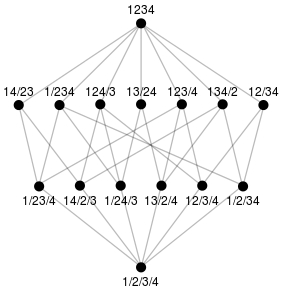
\includegraphics[scale=1]{Reticulo.jpg}   
	\caption{Retículo de subgrupos.}
	\label{Reticulo}
   \end{figure}

  \begin{theorem}[Teorema\IS de Lagrange]
   Si G es un grupo finito y H un subgrupo de G, entonces el número de elementos de H divide el número de elementos de G.
  \end{theorem}
  
  \begin{lemma}
   Sea $\varphi: G\rightarrow G$, son equivalentes:
   \begin{enumerate}
    \item $\varphi$  es inyectiva.
    \item $\varphi$  es biyectiva.
    \item $\varphi$  es sobreyectiva.
   \end{enumerate}
  \end{lemma}
  La demostración de este teorema es totalmente trivial. Con apoyarnos en que el conjunto G es finito, puede observarse que una de
  esas propiedades implica directamente las demas.
  
  \begin{lemma}
   Si $\varphi$  es un biyección y $A, B$ son subconjuntos de $G$:
   \begin{enumerate}
    \item $\text{card}(A)=\text{card}(\varphi(A))$
    \item $A=B \dimplies \varphi(A)=\varphi(B)$
    \item $\varphi(A\cap B)=\varphi(A)\cap\varphi(B)$
   \end{enumerate}
  \end{lemma}
  
  \begin{lemma}
   Sea G un grupo finito y $g \in G$, entonces $\varphi_{g}(x)=g\ast x$. Además, por la propiedad cancelativa, podemos ver que $\varphi_{g}$ es inyectiva.
   
   Además, por ser G finito, sabemos que $\varphi_{g}$ es biyectiva.
  \end{lemma}
  También podemos definir $\varphi_{g} H=\{g\ast h\tq h\in H\}$
  
  \begin{defn}[Clase\IS lateral]
  \[  gH=\varphi_{g}(H) \]
  \end{defn}

  \begin{corol} 
  \label{corol1}
  Extraemos las siguientes conclusiones:
   \begin{enumerate}
    \item $g \in gH$
    \item $\text{card}(H)=\text{card}(gH)$
    \item $H=gH \dimplies g \in H$ 
   \end{enumerate}
  \end{corol}

  \begin{proof}
   \begin{enumerate}
    \item $e \in  H$. Por tanto $g\ast e =g$ que por hipótesis está en $gH$.
    \item Se puede ver apoyándonos en los lemas anteriores puesto que H es finito.
    \item $\Rightarrow$):  $e \in H \implies e=gh$ con $h \in H$. Por lo tanto $h=g^{-1} \in H$ y entonces $g \in H$.\\
	  $\Leftarrow$):  $g \in H \implies g^{-1}\in H$ y todo elemento $h \in H$ cumple $h=g(g^{-1}h)\in H$.
   \end{enumerate}
  \end{proof}
  
  \begin{prop}
   Dados $g_{1}, g_{2}\in G$ y $H<G$, entonces \[ g_{1}H=g_{2}H \] y \[g_{1}H\cap g_{2}H=\emptyset \]
  \end{prop}
  
  \begin{proof}
   La intersección $g_{1}H\cap g_{2}H$ no será vacía si y sólo si $\exists\, h_{1},h_{2} \in H$ tal que $g_{1}h_{1}=g_{2}h_{2}$. Operando 
   \begin{gather*}
   h_{1}=g_{1}^{-1}g_{2}h_{2} \\
   h_{2}^{-1}h_{1}=g_{1}^{-1}g_{2}
   \end{gather*}
   
   Por ser $h_2$ y $h_1$ pertenecientes a $H$, tenemos que $g_{1}^{-1}g_{2} \in H$. Usando la propiedad 3 de (\ref{corol1}), nos queda que
    \[ g_{1}^{-1}g_{2}H=H  \] y por lo tanto \[ g_{2}H=g_{1}H \]
  \end{proof}
  
  \begin{example}
   Tomando el famoso grupo $D_{4}$, podemos obtener H=$\{1,g,g²,g³\}$; sH=$\{s,sg,sg²,sg³\}$
  \end{example}
  
  
  
  \subsection{Particiones}

  \begin{defn}[Relación\IS de equivalencia]
   Fijado un conjunto $G\neq\varnothing$. Una relación $\rel$ en $G$ es de equivalencia si cumple las siguientes propiedades:
  
   \begin{description}   
    \item[Reflexiva] $\forall x\in G \;  x\rel x$
    \item[Simétrica] $\forall x,y \in G\;  x\rel y \dimplies y \rel x$
    \item[Transitiva] $\forall x,y,z \in G\;  x\rel y \y  y\rel z \implies x\rel z$
   \end{description}  
  \end{defn}
 
  \begin{defn}[Partición]
   Familia de subconjuntos disjuntos dos a dos tales que su unión constituye el total. 
  \end{defn}
  
  Una partición define una relación de equivalencia y viceversa. Si $\rel$ es una relación de equivalencia en un grupo $G$, 
  definimos una partición en la que los subconjuntos (clases de equivalencia) son de la forma: \[ S_{x}=\{y\in G \tq x\rel y\} \]
  
  \begin{proof} Definimos una relación de equivalencia $\rel$ en $G$ a partir del grupo $H$:
  
   \[ g_{1}\rel g_{2} \Leftrightarrow g_{1}^{-1}g_{2}\in H \]  y comprobamos que, efectivamente, esta relación es de equivalencia.
   
   Tenemos $S_{e}=H$. Así $S_{g}$  o ya cubre junto con H todo G, o cojo otro $g^{'}$  y repito el proceso con $S_{g^{'}}$.
   Así formare una serie de grupos de la forma $S_{x}$  disjuntos dos a dos y cuya unión me da G.\\
   De esta forma podemos ver que $\card{G}=\card{H}  s$
  \end{proof}
  
  \begin{theorem}[Teorema\IS de Lagrange]
   Dado $g \in  G$, siendo $G$ un grupo finito, entonces $\ord{g}$ divide a $\card{G}$. 
  \end{theorem}
  
  Una interpretación rápida de este teorema es que si el cardinal de $G$ es primo, los únicos subgrupos que tiene $G$ son los triviales: $\gen{e}, G$
  
  \begin{theorem}
   Si el cardinal de $G$ es primo, entonces $G$ es cíclico. Además, si $|G|=n$, entonces \[ \ord{g} | \, n \; \forall g\in G\] y $g^n = e$.
  \end{theorem}
  
  \begin{example}
   Con ayuda de este teorema puede demostrarse el pequeño teorema de Fermat. 
   Definimos $\ent/p\ent=\{\bar{0},\bar{1}...,\bar{p-1}\}$.
   Si tomamos el grupo de las unidades de $\ent/p\ent$ tenemos $\{\bar{1}, \bar{2},....\bar{p-1}\}$ $\Rightarrow$
   $\bar{a}\in\ent/p\ent \wedge \bar{a}\neq 0 \Rightarrow a^{p-1}=\bar{1}$.
  \end{example}
  
  \begin{theorem}
   Si $|G|=p^{2}$  con $p$ primo entonces $\exists g \in G \tq \ord{g}=p$
  \end{theorem}
  
  \begin{proof}
   Tomamos $g\in G \y g\neq e$. Entonces sólo hay dos posibilidades, o bien $\ord{g}=p$ o bien $\ord{g}=p^{2}$. En el primer caso ya lo tenemos, y en el segundo tenemos que existe $g^p$ que tiene orden $p$.
  \end{proof}
  
  \begin{example}
   Por todo lo explicado anteriormente, si tomamos el anillo de polinomios $\ent/p\ent[x]$, tenemos \[ X^{p-1}-\bar{1}=
   \prod_{\bar{a}\in\ent/p\ent \wedge \bar{a}\neq 0}(x-\bar{a}) \]
  \end{example}
  
  \begin{theorem}[Teorema\IS de Lagrange]
   Dados $H<G$,  se cumple que \[ \exists a_{1},\dotsc,a_{r}\in G\tq G=a_{1}H \cup a_{2}H \cup \dotsb \cup a_{r}H\] y que \[ a_{i}H\cap a_{j}H=\emptyset \forall i\neq j\] 
   Es decir, $\card{G}=r\card{H}$
  \end{theorem}

  Definimos ahora otra relación a partir de $H<G$: \[ c\rel^{'}d \Leftrightarrow cd^{-1}\in H \]. La comprobación de que esto es una relación
  la omitiremos por ser trivial. En esta partición, el conjunto de elementos relacionados con d es: $Hd=\{hd\tq h\in H\}$
  
  \begin{defn}[Subgrupo\IS normal]
   Decimos que $H<G$  es un subgrupo normal si \[ gH=Hg \; \forall g \in G \]. Por tanto, si $G$ es un grupo abeliano, $H$ también lo será y cualquier  subgrupo será normal. Un subgrupo normal se expresa como $H\lhd G$.
  \end{defn}
  
  \begin{example}
   Tomamos $G=\ent$  y $H=4\ent$. 
   El subgrupo de los elementos que son equivalentes a n es nH=$\{n+4k\tq k \in \ent\}$.
   En este caso tenemos 4 subgrupos según esta condición: $\bar{0},\bar{1},\bar{2},\bar{3}$
  \end{example}
  
  Si $H\lhd G$  podemos definir una estructura de grupo en el subconjunto de clases, lo que se llamará el grupo cociente.
  
  \begin{defn}[Grupo\IS cociente] Sea $H \lhd G$. Definimos $G / H$ como el conjunto de todas las clases laterales izquierdas, es decir
  
  \[ G/H = \{ aH \tq a \in G\} \]
  \end{defn}
  
  
  Dados $g_{1}H$  y $g_{2}H$  podemos formar el conjunto $\{h_{1}\ast h_{2}\tq h_{1}\in g_{1}H \wedge h_{2}\in g_{2}H\}$. Si operamos   $g_{1}H\ast g_{2}H=(g_{1}\ast g_{2})H$  que es otra clase. Por tanto el grupo de clases es cerrado.
  
  El neutro sería la caja $H$ puesto que $gHH=gH$ para cualquier $g$ que escojamos. Además el inverso de $gH$ es $g^{-1}H$.
  
  Por último, vemos que $(g_{1}H\ast g_{2}H)\ast g_{3}H=g_{1}H\ast Hg_{2}\ast g_{3}H=g_{1}H\ast Hg_{3}\ast g_{2}H$, por ser G asociativo. Queda probado pues, que el conjunto de las clases de equivalencia, forma un grupo.
  
\begin{defn}[Índice\IS de un subgrupo] El índice de un subgrupo $H$ de $G$ es el \textit{tamaño relativo} de $H$ en $G$, el número de \textit{copias} de $H$ que llenarían $G$.  

Estrictamente, se define $[G:H]$ es el número de clases laterales de $H$ en $G$. Si $H$ y $G$ son finitos, entonces 

\[ [G:H] = \frac{\card{G}}{\card{H}} \]
\end{defn}
  
  \begin{theorem}
   \[ H< G \y [G:H]=2 \implies H \lhd G \]
  \end{theorem}
  
  \begin{proof}
   Por un lado tenemos que $g\notin H \implies gH= H^{c}$. Por otro lado, si tomamos la otra relación de equivalencia, a partir de $g \notin H obtenemos Hg=H^{c}$.
   
   Uniendo estos dos ejemplos, donde mantenemos H como una mitad en ambos, tenemos Hg=gH. Por tanto H es un subgrupo normal.
   
   Guille: Me lo creo pero me convence cero. ¿Qué es $H^c$? ¿Cuál es la otra relación de equivalencia?
  \end{proof}
  
  \begin{lemma}
   Dadas dos particiones formadas por los subconjuntos $aH$ y $Ha$ para un elemento $a \in G$ y con $H <G$, podemos definir dos aplicaciones $\pi$ y $\pi '$ que lleven cada elemento de G a su respectiva caja \textit{¿qué es una caja?}:
   \[ \appl{\pi}{G}{G/H} \]
   \[ \appl{\pi'}{G}{G/H} \]
   
   Tenemos entonces que:
   
   \[ H \text{subgrupo normal} \implies a_iH = Ha_i \]
   \[ H \text{subgrupo normal} \implies \pi \ =\ \pi ' \]
   
   Además, si H es normal
   \begin{enumerate}
	\item Podemos definir una operación en el conjunto cociente.     
	\item $\appl{\pi}{G}{G/H}$ es compatible con las operaciones.
   \end{enumerate}
  \textit{Pues vale.}
  \end{lemma}
  
\begin{defn}[Centro de un grupo]
	Llamamos centro del grupo $G$ al grupo formado por todos los elementos que conmutan con todos los elementos de $G$.:\\
	\[ Z(G) = \{ a\in G\tq a\ast g = g\ast a\ \forall g\in G\} \]
	Además, tenemos que:
	\[ aZ(G)=Z(G)a \implies Z(G)\lhd G \]
  \end{defn}  
  
  \begin{example}
	Sea $Q$ el grupo formado por las raíces cuartas de 1:
	\[ Q = \{ 1, i, j, k, -1, -i, -j, -k\} \] 
	
	Podemos ver que $Q$ se genera a partir de los elementos $i, j, k$: $Q = \gen{i,j,k}$.
	Además vemos que $-1$ conmuta con todos los elementos del grupo: $-1 \in Z(Q)$
	Analizamos el retículo del grupo y vemos que esta formado por los subgrupos:
	
	\begin{gather*}
	Orden\; 1 = \{ 1\}\\
	Orden\; 2 = \{ 1, -1\} \\
	Orden\; 4 = \{ 1, i, i^2, i^3\},\
			  \{ 1, j, j^2, j^3 \},\
			  \{ 1, k, k^2, k^3 \}.\\
			  \end{gather*}
			  
		  
	El grupo no es abeliano, sin embargo, todos sus subgrupos son normales porque todo subgrupo $H<G$ de índice 2 (es decir, el conjunto de clases $G/H$ tiene dos elementos) es normal.
	
  \end{example}
  
 
 Dados un grupo G y un subconjunto no vacío S, defino $S^{-1}=\{s^{-1}\tq s\in S\}$. Dados $S_{1},S_{2}<G$, defino  \[ (S_{1}\ast S_{2})^{-1}=\{s_{1}\ast s_{2}\tq s_{1}\in S_{1} \wedge s_{2}\in S_{2}\} \]
 
 que operando, nos queda que 
 
 \begin{align*}
 (S_1 \ast S_2)^{-1} &= \{s_{1}^{-1}\ast s_{2}^{-1}\tq s_{1}\in S_{1} \wedge s_{2}\in S_{2}\}\\
 &= \{s_{1}^{-1}\ast s_{2}^{-1}\tq s_{1}^{-1}\in S_{1}^{-1} \wedge s_{2}^{-1}\in S_{2}^{-1}\} \\
 & =S_{2}^{-1}\ast S_{1}^{-1}
 \end{align*}
 
 Sea H un subgrupo de G, entonces $H^{-1}=H$.
 
 \begin{theorem}
  Fijado un grupo G y $H_{1}, H_{2}$  subgrupos de G entonces: $H_{1} \lhd G \implies H_{1}\ast H_{2}<G$. 
 \end{theorem}
 
 \begin{proof}
  Sabemos que $H_{1}\ast H_{2}=H_{2}\ast H_{1}$. Para ver que $H_{1}\ast H_{2}<G$  hay que comprobar que está
  \begin{enumerate}
   \item Cerrado por la operación: $(H_{1}\ast H_{2})\ast (H_{2}\ast H_{1})=H_{1}\ast (H_{2}\ast H_{2})\ast H_{1}=H_{1}\ast H_{1}\ast H_{2}\ast H_{2}=H_{1}\ast H_{2}$
   \item Todo elemento tiene inverso, es decir: $\alpha\in H_{1}\ast H_{2}\Rightarrow \alpha^{-1}\in H_{1}\ast H_{2}$. Pero entonces tenemos:
   $\alpha^{-1}\in (H_{1}\ast H_{2})^{-1} = H_{2}^{-1}\ast H_{1}^{-1}=H_{2}\ast H_{1}=H_{1}\ast H_{2}$ que también contiene a $\alpha$ \textit{por ejemplo.}
  \end{enumerate}

 \end{proof}

 \begin{example}
  Tomamos el ya famoso grupo $D_{4}=\{1,g,g^{2},g^{3}, s, sg, sg^{2}, sg^{3}\}=\gen{s,g}$.
  
  Dentro de este grupo, el elemento 1 tiene orden dos, los elementos $g$, $g^{3}$  tienen orden 4 y el resto, 2.
  \begin{gather*}
  Z(D_{4})= \{\alpha\in D_{4} \tq \alpha\beta=\beta\alpha \ \forall \beta \in D_{4}\}= \\
  = \{\alpha\in D_{4}\tq \alpha s = s\alpha \wedge \alpha g = g\alpha\}=\{1, g^{2}\}=\gen{g^{2}}
  \end{gather*} 
  
  Este subgrupo es normal.
  
  Para contruir el retículo de subgrupos tomamos, en primer lugar, el único grupo de un elemento: 
  \[ \{1\} \]
  Ahora tomamos los grupos de orden dos, que serán todos aquellos generados por elementos que tienen orden dos:\\
  \[ \gen{sg^{3}}, \gen{sg}, \gen{g^{2}}, \gen{s}, \gen{sg^{2}} \]
  
  Los subgrupos de orden cuatro son los formados por elementos de orden 4 más los obtenidos al combinar el centro con los demás subgrupos de orden 2:
  \[ \{1,g,g^{2},g^{3}\}, \ \gen{g}, \ \{1, g^{2}, s, sg^{2}\} \]
 \end{example}
 

 \begin{proof}
 \begin{enumerate}
  \item $\Rightarrow$  Obvio, tan obvio como que $D_4$ le apasiona al profesor.
  \item $\Leftarrow$\\
  $aHa^{-1} \subset H \ \Rightarrow \ a^{-1}Ha\subset H.$. Por tanto $a^{-1}aHa^{-1}a \subset a^{-1}Ha \ \Rightarrow \ a^{-1}Ha \subset  a^{-1}Ha \Rightarrow \ H \subset a^{-1}Ha$.
  Contención a derecha e izquierda implica igualdad.
 \end{enumerate}
 \end{proof} 
 
 \subsection{Homomorfismos de grupos}
 \begin{defn}[Homomorfismo]
 Sea f $\appl{f}{(G_1, \cdot )}{(G_2, \ast )}$. $f$ es un homomorfismo de grupos si 
 \[ f(a\cdot b) = f(a)\ast f(b) \]
 \end{defn}
 
 \begin{example}
 Si consideramos la aplicación $\appl{\pi}{G}{G/N}$ que lleva los elementos de $G$ a su respectivo conjunto cociente, la función sobreyectiva $\pi$ es un homomorfismo de grupos si $N\lhd G$.
 \end{example}
 
 \begin{props} 
 Si $\appl{f}{G_1}{G_2}$ es un homomorfismo de grupos, entonces
 \begin{enumerate}
 \item $f(e_1) = e_2$ con $e_1$ neutro de $G_1$ y $e_2$ neutro de $G_2$
 \item $f(x^{-1}) = f(x)^{-1}$
 \end{enumerate}
 \end{props}
 
 \begin{proof} 
 1) 
 \begin{align*}
 e_1\cdot e_1 &= e_1 \\
 f(e_1)& =f(e_1\cdot e_1) = f(e_1)\ast f(e_1) \\
 f(e_1) &= e_2 \ast e_2 = e_2
 \end{align*}

 2) \begin{align*}
 f(x\cdot x^{-1}) &= f(e_1) = e_2 \\ 
 f(x)\ast f(x^{-1}) &= e_2 \\
  f(x^{-1}) &= f(x)^{-1}
  \end{align*}
 
 \end{proof}
 
 

\begin{remark} Si $G$ es un grupo finito \[\ord{f(a)}\ |\;\ord{a}\, \forall a \in G_1 \] \end{remark}

\begin{lemma}
La composición de dos homomorfismos de grupos es un homomorfismo de grupos.
\end{lemma}

\begin{defn}[Núcleo\IS de un homomorfismo]
Dado $\appl{f}{G_1}{G_2}$ el núcleo de $f$ se define como 

\[ \ncl{f} = \{ a\in G_1 \tq f(a) = e_2\} \]

con $e_2$ el elemento neutro de $G_2$. 

Además, se cumple que $\ncl f = \{ e_1 \}$ si y sólo si $f$ es inyectiva.
\end{defn}

\begin{theorem}
 Sea $\appl{f}{G_1}{G_2}$ un homomorfismo de grupo. Entonces $\ncl f$ y $\img f$ son subgrupos de $G_1$ y $G_2$ respectivamente, con $\ncl f$ el núcleo de la aplicación y $\img f$ la imagen de la misma.
 \end{theorem}
 
 \begin{proof} Empezamos demostrando que el núcleo es un subgrupo.
 \begin{gather*}
  \ncl f < G_1 \\
 e_1 \in \ncl f \\
 x, y \in \ncl f \implies xy^{-1}\in \ncl f \\
 f(xy^{-1}) = \underbrace{f(x)}_{e_2} \underbrace{f(y)^{-1}}_{e_2^{-1}} = e_2
 \end{gather*}
 
Pasamos ahora a demostrarlo con la imagen.

\begin{gather*}
\img f < G_2 \\
 e_2\in \img f \implies e_2 = f(e_1)\\
 a\in \img f \implies a^{-1}\in \img f\\
 \exists \alpha \in G_1 \tq a=f(\alpha ) \implies a^{-1} = (f(\alpha ))^{-1} = f(\alpha ^{-1})
 \end{gather*}
 
 \end{proof}

\begin{defn}[Epimorfismo]
Sea $\appl{f}{G_1}{G_2}$ un homomorfismo de grupos. Entonces diremos que $f$ es un epimorfismo si $\img f = G_2$.
\end{defn}

\begin{defn}[Monomorfismo]
Sea $\appl{f}{G_1}{G_2}$ un homomorfismo de grupos. Entonces diremos que $f$ es un monomorfismo si $\ncl f = \{ e_1\} $
\end{defn}

\begin{lemma} Sea $\appl{f}{G_1}{G_2}$ un homomorfismo de grupos, entonces se tiene que

\[ \ncl f \lhd G_1 \]
\end{lemma}

\begin{proof} Recordemos la definición de subgrupo normal:
\[ H \lhd G_1 \dimplies \forall a\in G_1\ aHa^{-1}\subset H \]
En este caso, tenemos que
\[ \forall a\in G_1\ a\ncl{f}a^{-1} = \{aha^{-1} \tq h\in \ncl{f} \} \]

Si tomamos $f\left(a\ncl{f}\inv{a}\right)$, vemos que es igual a \[ f(a) f(\ncl{f}) f(\inv{a}) = \alpha e_2 \inv{\alpha} = e_2 \]
\end{proof}

\begin{remark}El único homomorfismo de $\ent/n\ent$  en $\ent$, y en general de un grupo finito a los enteros, es el trivial. Esto se debe
a que dado $a\in\ent/n\ent$, ord(a)=$\alpha$, pero $\ord{f(a)}$ será infinito, salvo que $f(a)=0$.\end{remark}
  
\begin{lemma} Si $N\lhd G$ entonces $G/N$ tiene estructura de grupo y $\appl{\pi}{G}{G/N}$  (homomorfismo que manda cada
elemento a su grupo cociente)  es un epimorfismo.
\end{lemma}

\begin{lemma} Dado $\appl{f}{G_1}{G_2}$, con $N=\ncl{F}$ y $N \lhd G$, entonces
\[ b\in aN \dimplies  a^{-1}b\in N \dimplies f(a^{-1}b)=e_2 \ \dimplies f(a)^{-1}f(b)=e_2 \ \dimplies f(a)=f(b) \]
\end{lemma}

\begin{defn}[Isomorfismo]
Diremos que f es un isomorfismo si existe un homomorfismo de grupo $\appl{g}{G_2}{G_1}$  de tal forma que f$\circ$g=id. El hecho de
que f sea isomorfo, implica, por definición, que f es un homomorfismo y que es biyectivo.
\end{defn}

Partiendo de $\appl{f}{G_1}{G_2}$  un homomorfismo de grupos, se cumple que:
\begin{enumerate}
 \item $H<G_1 \ \Rightarrow \ f(H)<G_2$
 \item $H_2<G_2 \ \Rightarrow \ f^{-1}(H_2)<G_1$
 \item $H_2 \vartriangleleft G_2 \ \Rightarrow \ f^{-1}(H_2)\vartriangleleft G_2$
 \item f sobreyectiva y $H_1 \vartriangleleft G_1 \ \Rightarrow \ f(H_1)\vartriangleleft G_2$
\end{enumerate}
\begin{proof}
Recordamos que dado S un suconjunto de G, para probar que S es un subgrupo bastaba con ver que $S \neq \varnothing$  y que $xy\in S \ \Rightarrow \ y^{-1}x\in S $
 \begin{enumerate}
  \item f(H) $\neq \varnothing$\\
  $a,b\in f(H) \tq a=f(x) y b=f(y) \Rightarrow \ b^{-1}a=f^{-1}(y)*f(x)=f(y^{-1}x)\in H$
  \item $f^{-1}(H)\neq \varnothing$\\
  $f(x)=a, f(y)=b \Rightarrow \ xy\in f^{-1}(H_2) \Rightarrow \ y^{-1}x=f(y^{-1}x)\in f^{-1}(H_2)$
  \item Si tomo $\appl{\varphi}{G_2}{G_2/H_2}$  un homomorfismo de grupos. Dado que la composición de homomorfismos es otro homomorfismo, 
  tenemos que $\varphi \circ f$  es un homomorfismo. Además, el núcle de $\varphi$  es $H_2$, por lo que el núcleo de la composición sera $f^{-1}(H_1)$.
  Por otro lado, ya hemos visto que el núcleo de un homomorfismo es un subgrupo normal del grupo de partida. Por tanto $f^{-1}(H_1) \vartriangleleft G_1$
 \end{enumerate}
 \end{proof}

\begin{defn}[Isomorfismo]
Un homomorfismo de grupos $\appl{f}{G_1}{G_2}$ es un isoformismo si existe un homomorfismo de grupos $\appl{g}{G_2}{G_1}$ tal que $g\circ f = id_{G_1}$ y $f\circ g = id_{G_2}$. 
\end{defn}


\begin{remark} Dados dos grupos $G_1$ y $G_2$, $\appl{f}{G_1}{G_2}$ es un isomorfismo de grupos si y sólo si f es un homomorfismo y es una biyección de conjuntos.
\end{remark}

\begin{lemma}
Sea $\appl{f}{G_1}{G_2}$, entonces:
\begin{enumerate}
\item Si $H_1$ es un subgrupo de $G_1$, $f(H_1)<G_2$
\item Si $H_2 < G_2$, entonces $f^{-1}(H_2)<G_1$
\item Si $H_2 \lhd G_2$, $f^{-1}(H_2)\lhd G_1$
\item Si $f$ es sobreyectiva y $H_1\lhd G_1$, tenemos que $f(H_1)\lhd G_2$
\end{enumerate}
\end{lemma}

\begin{proof}
\paragraph{Propiedad 1}
\begin{gather*}
e_2 \in f(H_1)\\
x, y\in f(H_1) \implies xy^{-1}\in f(H_1)\\
x=f(a);\; y = f(b);\; a, b\in H_1\\
xy^{-1}=f(a)f(b)^{-1} = \underbrace{f(ab^{-1})}_{H_1} \in f(H_1)
\end{gather*}

\paragraph{Propiedad 2}
\begin{gather*}
e_1 \in f^{-1}(H_2)\\
a, b \in f^{-1}(H_2) \implies ab^{-1} \in f^{-1}(H_2)\\
f(a) \in H_2;\; f(b) \in H_2 \implies \underbrace{f(ab^{-1})}_{f(a)f(b)^{-1}}\in H_2
\end{gather*}

\paragraph{Propiedad 3}
$f^{-1}(H_2) = N(\pi \circ f)$. Como $f^{-1}(H_2)$ es el núcleo de h de g entonces $f^{-1}(H_2)\lhd G_1$.
\end{proof}


Sea $\appl{f}{G_1}{G_2}$ un homomorfismo de grupos, y $f$ sobreyectiva (es decir, un \textit{epimorfismo})
vamos a analizar el retículo de subgrupos de $G_2$.\\
Fijado un subgrupo $H_2<G_2$ le asociamos un subgrupo $f(H_2)<G_1$. Asociamos al retículo de subgrupos de $G_2$ subgrupos de $G_1$ que contienen al núcleo $N(f)$.
\begin{theorem}
Es posible identificar el retículo de subgrupos de $G_2$ con los subgrupos de $G_1$ que contienen al núcleo $N(f)$
\end{theorem}

\obs Sea $\appl{f}{G_1}{G_2}$ sobreyectiva. $H$ subgrupo de $G_1$ que contiene al núcleo $N(f)$. Entonces $H = f^{-1}(f(H))$
Como $f(H)$ es un subgrupo de $G_2$ la observación indica que todo subgrupo de $G_1$ que contiene al núcleo es de la forma $f^{-1}(K)$ para algún subgrupo K de $G_2$

\begin{example}
El retículo de subgrupos de $Q/{\{ -1, 1 \} }$ se identifica con los subgrupos de $Q$\footnote{Grupo de cuaterniones, osea, raíces cuartas de uno.} que contienen al núcleo $\{ 1, -1\} $.
\end{example}

\begin{defn}[Grupos\IS isomorfos]
Dos grupos son isomorfos si existe un isomorfismo entre ellos.
\end{defn}

\begin{theorem}
Si $\appl{f}{G_1}{G_2}$ es un homomorfismo de grupos entonces $Img(f)$ (subgrupo de $G_2$) es isomorfo al grupo cociente $G_1/{N(f)}$\footnote{Recordad que $\ncl f \lhd G_1$}
\end{theorem}

\begin{example}
Si tenemos la aplicación 
\begin{gather*}
\appl{h}{\mathbb{Z}}{\mathbb{C}^*}\\
1 \longrightarrow i\\
k\longrightarrow ik\\
\end{gather*}

$\ncl f = 4\mathbb{Z} < \mathbb{Z}$\\
$Img(f) = \{1, i, -1, -i \}$
Tenemos que $\{ 1, i, -1, -i \}$ es isomorfo al grupo $(\mathbb{Z} /4\mathbb{Z}, +)$
\end{example}

\begin{defn}[Biyección]
 Un homomorfismo $\appl{f}{G_1}{G_2}$ es una biyección si \\
 $\exists \ \appl{h}{G_2}{G_1} \tq \ f\circ h =id \ en \ G_1 \ y\ h \circ g = id \ en \ G_2$.
\end{defn}
Para decidir si un homomorfismo de grupo $\appl{f}{G_1}{G_2}$  es un isomorfismo o no, basta con ver si $f$  es una biyección.\\

Siendo $\appl{f}{G_1}{G_2}$ un isomorfismo se cumple que:\\
\begin{enumerate}
 \item ord(f(g))=ord(g)
 \item A partir de f se establece una identificación con el retículo de subgrupos
 \item Dos grupos isomorfos comparten propiedades hasta el punto de no poderlos distinguir. (Equivalente a cuando no distinguíamos
 dos espacios vectoriales isomorfos).
\end{enumerate}

\begin{theorem}[Teoría de isomorfismos]
 Siendo N(f)$\lhd$G, con $\appl{f}{G_1}{G_2}$ y $\appl{\pi}{G_1}{G_1/N(f)}$se cumple:
 \begin{enumerate}
  \item $\exists \appl{f^{'}}{G_1}/N(f){G_2} \ \tq f=f^{'}\pi$
  \item $f^{'}$  es un homomorfismo de grupos
  \item $f^{'}$  es inyectiva.
  \item Img(f)=Img($f^{'}$)
 \end{enumerate}
\end{theorem}
\begin{proof}
 \begin{enumerate}
  \item Si tomamos $f^{'}(\bar{a})=f(a)$  tenemos que ver que está bien definido, es decir, que no depende del representante escogido.\\
  $\bar{a^{'}}=\bar{a} \Leftrightarrow a^{'}N(f)=aN(f) \ \Leftrightarrow a^{'}\in N(f)a \ \Leftrightarrow \ f(a^{'})=f(a)$
  \item Probamos ahora que es un homomorfismo de grupos:\\
  $ f^{'}(\bar{a}\bar{b})=f^{'}(\bar{ab})=f(ab)=f(a)f(b)$
  \item Veamos ahora la inyectividad\\
  $\bar{a}\in N(f) \Leftrightarrow f^{'}(\bar{a})=e_2 \ \Leftrightarrow \ f(a)=e_2 \ \Leftrightarrow \ a\in N(f) \ \Leftrightarrow \ \bar{e}=bar{a}$
  \item Se cumple por ser $\appl{\pi}{G_1}{G_1/N(f)}$.
 \end{enumerate}
\end{proof}

\begin{theorem}[Teorema 1 de isomorfía]
 Si $\appl{f}{G_1}{G_2}$  es un isomorfismo de grupos sobreyectivo, entonces $G_2$  es isomorfo al grupo $G_1/N(f)$.
\end{theorem}
\begin{proof}
 Sabemos que $f^{'}$  es un homomorfismo inyectivo y como $\pi$  es sobreyectivo Img(f)=Img($f^{'}$)=$G_2 \ \Rightarrow f^{'}$ sobreyectiva.\\
 Por tanto, $f^{'}$  es una biyección.
\end{proof}
\begin{corol}
 Si G es cíclico de orden n, entonces G es isomorfo a ($\mathbb{Z}/n\mathbb{Z}$, +)
\end{corol}

\begin{notacion}
$G_1 \simeq G_2$ es decir que $G_1$ isomoforfo a $G_2$.
\end{notacion}

\begin{example}
Si tenemos un grupo $G$ cíclico, tal que el orden de $G$ es $n$ entonces sabemos que
$\exists a \in G \tq ord(a) = |G|$
Si tomamos el homomorfismo siguiente:\\
$$\appl{f}{\mathbb{Z}}{G}$$\\
$$k \longrightarrow a^k$$\\
es sobreyectiva y su núcleo son los multiplos de $n$ ($n\mathbb{Z}$)
El primer teorema de isomorfía dice que $G \simeq \mathbb{Z}/\ncl f  = \mathbb{Z}/n\mathbb{Z}$
\end{example}

Otra manera de ver el teorema de isomorfía es el siguiente.
\begin{theorem}[Teorema 1 de isomorfía (II)]
Sea $\appl{f}{G}{G'}$ un homomorfismo de grupos, entonces $Img(f) \simeq G/\ncl(f)$
\end{theorem}

Esta es una visión más general, que dice que aunque f no sea sobreyectiva, la imagen de f es isomorfa a $G/\ncl(f)$

\begin{lemma}
 Dado un homomorfismo de grupos $\appl{f}{G}{G'}$  con N(f)$\subset$G.\\
 Sea $N_1 \vartriangleleft N(f) \vartriangleleft G$. Entonces existe $\bar{f}$, homomorfismo de grupos tal que $\bar{f}\circ\pi=f$.\\
 Se tiene ademas que Im($\bar{f}$)= Im(f) por ser $\pi$  sobreyectiva.
\end{lemma}
\begin{proof}
 La demostración de este lemma es idéntica a la de la teoría de isomorfismos. Sólo hay que cambiar N(f) por $N_1$.
\end{proof}

Vamos a ver ahora cuantos homomorfismos existen de la forma $\appl{f}{\mathbb{Z}}{G}$.\\
En general, existen tantos homomofismos como elementos tenga el grupo G. Para ver esto, vamos a construirlos.\\
Si al 1 le asociamos un elemento $a \in$G, a cada elemento k le asociamos $a^{k}\in$G. Por tanto, tenemos homomorfismos como valores
podamos asociar al 1 y tenemos tantos valores posibles como elementos de G.\\
\\
Ahora vemos que pasa si tomamos $\appl{f}{\mathbb{Z}/n\mathbb{Z}}{G}$. \\
En este caso el homomorfismo queda determinado por f($\bar{1}$) porque
f($\bar{2}$)=f($\bar{1}+\bar{1}$)=f($\bar{1}$)f($\bar{1}$). Además ord(f($\bar{1}$)/ord($\bar{1}$)=n\\
El lema anterior nos permite ver que el recíproco de esta afirmación es cierto.\\
\begin{proof}
Construyo $\appl{f}{\mathbb{Z}}{G}$  con g(1)=$a\in G$ con N(g)=n$\mathbb{Z}$  y n=ord(a)
Puedo aplicar el lema anterior $\Rightarrow \exists \appl{f}{\mathbb{Z}/n\mathbb{Z}}{G} \ \tq f(1)=a$. (Esta sería la $\bar{f}$ del lema).
\end{proof}

Por tanto, para ver cuántos homomorfismos hay de la forma $\appl{f}{\mathbb{Z}/n\mathbb{Z}}{A}$, tengo que ver cuántos elementos
de A tienen un orden que divida a n (para mandar allí el $\bar{1}$)\\

\begin{lemma}
 Dados $N\vartriangleleft N' \vartriangleleft G$, puedo dividir G en "cajas" a partir de la relación de equivalencia basada en N. Es decir,
cada "caja" tendrá los elementos de la forma g$N$  con g$\in G$. Por otro lado, puedo hacer este mismo proceso con $N'$.\\
Se observa pues, que las cajas de $N'$  esta formada por la unión de cajas de $N$. Por tanto tenemos que $N'/N \vartriangleleft G/N$.\\
\end{lemma}

\begin{theorem}[Teorema 2 de isomorfía]
 Dados $N_1\vartriangleleft N_2 \vartriangleleft G$  se tiene que:
 \[ (G/N_1)/(N_2/N_1)\backsimeq G/N_2\]
 Donde $\backsimeq$  denota isomorfo.
\end{theorem}

\begin{proof}
 Como $N\vartriangleleft G  \wedge  N_1 \lhd N_2$, aplicando el lema 1.58 tenemos que existe un epimorfismo $\appl{\bar{\pi}}{G/N_1}{G/N_2}$.\\
 Aplicando el teorema 1 de isomorfía tenemos que $G/N_2 \backsimeq (G/N_1)/N(\bar{\pi})$. Si logramos probar que el núcleo de $\bar{\pi}$ 
 es lo mismo que $N_2/N_1$  ya estará finlizada la demostración.\\
 El núcleo de la aplicación $\bar{\pi}$  son aquellos elementos de $G/N_1$  que van a $\bar{e}$, es decir, aquellos elementos que pertenecen a $N_2$.
 Si una clase de tipo $\bar{g}\in N_2 \Rightarrow g \in N_2$. Por tanto el núcleo está formado por aquellas clases de equivalencia de elementos pertenecientes a $N_2$.
 Es decir, el núcleo es $N_2/N_1$. (Si no lo ves claro piensa que las clases de elementos de G se representaban como $G/N_1$, ahora es lo mismo pero
 no son elementos de G sino de $N_2$  porque quiero el núcleo.).
\end{proof}

\begin{example}
 Vamos a ver un ejemplo de como construir homomorfismos.\\
 Supongamos que quiero construir un homomorfismo $\appl{f}{D_3}{G}$.\\
 Por lo explicado anteriormente, este homomorfismo quedará determinada por la imagen de los generadores de $D_3$. Por tanto,
 basta con escoger dos elementos de $G$  y asignarlos $f(s)=\alpha, \ f(g)=\beta$  de tal forma que: ord($\alpha$)/ord($f(s)$) y ord($\beta$)/ord($f(g)$).\\
 Pero además, estos dos elementos deben cumplir la última propiedad que me definía $D_3$: $f(s)f(g)=(f(g))^{-1}f(s)$
\end{example}

\begin{defn}
Dados H, K dos subgrupos de G, siendo H un subgrupo normal, HK es el menor subgrupo de G que contiene a ambos.
\end{defn}
 Si tenemos $H \vartriangleleft G \ \appl{\pi}{G}{G/H}$, dado un $\bar{K} < G/H, \  H \subset \ \pi^{-1}(\bar{K}) < G $, por ser $e_2 < \bar{K}$\\
 Por otro lado, todo subgrupo de G que contiene a H cumple que $K=\bar{\pi}^{-1}(\bar{\pi}(K))=$.
 
 \begin{example}
  Dados $H=d_1\mathbb{Z}, \ , K=d_2\mathbb{Z}$, HK es el menor subgrupo que los contiene, por tanto $HK=d\mathbb{Z}$, con d=m.c.d.($d_1, d_2$).
 \end{example}

 \begin{theorem}
  Todo subgrupo de $\mathbb{Z}/n\mathbb{Z}$  es cíclico de la forma <$\bar{d}$>, donde d divide a n y ord(<$\bar{d}$>)=n/d.
 \end{theorem}
\begin{example}
 Tenemos $\bar{K}\in \mathbb{Z}/n\mathbb{Z}$  con subgrupos <$\bar{d_1}$>, <$\bar{d_2}$>,..., <$\bar{d_r}$> con r divisor de n.\\
 Si ahora genero <$\bar{K}$> quiero ver con que subgrupo coincide.\\
 Tomo $\appl{\pi}{\mathbb{Z}}{n\mathbb{Z}}$.\\
 Sabemos que $n\mathbb{Z}=N(\pi) \subset \pi^{-1}(\bar{K})$  y también sabemos que $\bar{K} \in \pi^{-1}(\bar{K}$. Es decir,
 la contraimagen debe contener a k y a n. Por tanto debe contener a k$\mathbb{Z}$  y a n$\mathbb{K}$, por lo que es el subgrupo
 d$\mathbb{Z}$  con d=m.c.d.(k,n).\\
 $\pi(\pi^{-1}(\bar{K}))=\pi(d\mathbb{Z})=<\bar{d}>$, que tiene orden n/d.
\end{example}

Si G es un gurpo cíclico de orden n, entonces es isomorfo a $\mathbb{Z}/n\mathbb{Z} \Rightarrow$  todo subgrupo de G es cíclico y 
tiene tantos subgrupos como divisores positivos tiene n.

\begin{theorem}
 $a\in G \wedge ord(a)=n \ \Rightarrow ord(a^{k})=\frac{ord(a)}{d}$, con d=m.c.d.(n,k)
\end{theorem}

\begin{proof}
 Construyo un homomorfismo $\appl{f}{\mathbb{Z}}{G}$  tal que f(1)=a. \\
 Así tenemos que $<a>\simeq \mathbb{Z}/n\mathbb{Z} \ n=ord(a)$.\\
 Este isomorfismo me lleva $a^{h}\textrightarrow \bar{k}$  y ord($a^{k}$)= ord($\bar{k}$) y  aplicando el teorema anterior tenemos
 que ord($\bar{k}$)=n/d con d=m.c.d.(n,k).
\end{proof}

\begin{defn}[Automorfismo]
 Isomorfismo que nos lleva un conjunto en sí mismo. Aut(G) es el conjunto de automorfismos de G.
\end{defn}

\begin{example}
 Vamos a buscar Aut($\mathbb{Z}$)\\
 g(1)=1 y g(1)=-1 son todos los automorfismos posibles.\\
 Así tenemos Aut($\mathbb{Z}$)=$\{1,-1\}$=$\{f, f^{-1}\}$. Ambas son expresiones del conjunto de automorfismos de $\mathbb{Z}$. Ambas
 consituyen grupos pero con distintas operaciones asociadas. Estas operaciones son la suma y la composición respectivamente.
\end{example}

\begin{example}
 Vamos a buscar Aut($\mathbb{Z}/n\mathbb{Z}$)\\
 Como ya hemos visto, para encontrar homomorfismos de $\mathbb{Z}/n\mathbb{Z}$  basta con definir f($\bar{1}$) = g con ord(g)/n=ord($\bar{1}$).\\
 Definimos por tanto los homomorfismos de grupo $\appl{f}{\mathbb{Z}/n\mathbb{Z}}{\mathbb{Z}/n\mathbb{Z}}$  de la forma f($\bar{1}$)=$\bar{g}$, con 
 ord($\bar{g}$)/n.\\
 Estos homomorfismos serán isomorfismos si  ord($\bar{g}$)=n, lo cual ocurre si $\bar{g}\in U(\mathbb{Z}/n\mathbb{Z}) \ \Leftrightarrow g \ coprimo \ con\ n$\\
 Como la composición de isomorfismos es otro isomorfismo, vuelve a cumplirse que Aut($\mathbb{Z}/n\mathbb{Z}$)  es un grupo.
\end{example}

Para que una aplicación de un conjunto finito en sí mismo sea una biyección, basta con ver que cumple la propiedad inyectiva o sobreyectiva
ya que las siguientes son consecuencia directa. Es decir, por ser finito, si la aplicación es inyectiva, no le queda otra que ser
también sobreyectiva y por tanto, biyectiva.\\

Sea $\{1,...n\}$=$S_1\coprod S_2\equiv unión \ disjunta$  y sea $\alpha$  una biyección que fija los elementos de $S_1$  y $\beta$
otra que fija los elementos de $S_2$. En tal caso, estas biyecciones conmutan.\\
En general, si $\alpha$,  $\beta$  son biyecciones disjuntas se cumple que:
\begin{enumerate}
 \item $\alpha \circ \beta = \beta \circ \alpha$
 \item $\alpha^{k}, \beta^{l}$  son también biyecciones disjuntas, ya que siguen dejando fijos los elementos de `$S_1$  y $S_2$  respectivamente.
\end{enumerate}

\begin{defn}[Ciclo]
Fijado ($i_1, i_2,...,i_r$)$\subset$(1,2,3,...n), un ciclo es una biyección que lleva cada elemento $i_i$  al siguiente $i_{i+1}$, y deja
fijos los demás elementos de (1,2,3,...n).
\end{defn}

\begin{theorem}
 Toda biyección puede expresarse de forma única como la composición de biyecciones disjuntas
\end{theorem}
\begin{proof}
 Dada una aplicación, reconozco sus ciclos y la combinación de ellos me dará la aplicación. En realidad estoy reescribiendo los
 cambios que realiza la aplicación en forma de ciclo y dejando los elementos que la aplicación dejaba quietos igual. \\
 Por ser los ciclos biyecciones disjuntas, el efecto de uno no interfiere en otro.\\
\end{proof}
Veamos esto más claro con un ejemplo.
\begin{example}
 Tenemos la aplicación $\sigma$=(2,3,1,4,6,5,7,9,8,10). Vamos a buscar sus ciclos. Para ello, cojo un elemento y voy viendo donde
 lo mandan sucesivas aplicaciones de la función hasta volver a mi punto de partida.\\
 Empezamos con el 1. Aplicando sucesivamente la aplicación, observo las siguientes transformaciones: 1$\Rightarrow$2$\Rightarrow$3$\Rightarrow$1. Ya
 tenemos un ciclo. Este ciclo será representado como (1,2,3) según la notación indicada en la definición de estos ciclos.\\
 Ahora tomo otro elemento que no esté incluido ya en este ciclo. 4 $\Rightarrow$4. Este sería un ciclo con un único elemento, sería
 la identidad, que no es necesario representar.\\
 Tomo ahora 5 $\Rightarrow$ 6 $\Rightarrow$ 5. Tenemos aquí un ciclo de orden dos (5,6)\\
 Tomo ahora 7 y veo que estamos en el mismo caso que el 4.\\
 Tomo el 8 $\Rightarrow$ 9$\Rightarrow$8. Tenemos otro ciclo de orden dos (8,9).\\
 El 10 nos queda invariante.\\
 Por tanto tenemos que nuestra aplicación $\sigma$ = (1,2,3)(5,6)(8,9). Es decir, si a un conjunto de 10 elementos ordenados le aplico
 estos tres ciclos, obtengo el mismo resultado que aplicándole directamente la aplicación $\sigma$.
\end{example}

Ahora vamos a demostrarlo.

\begin{proof}
Fijamos un $\sigma \in S_n$. Sea $X = \{ 1,2,\hdots ,n\} $.\\
Vamos a crear una partición definiendo la siguiente relacion:\\
$a,b \in X$, $aRb$ si $\sigma ^i(a) = b$ para algun $i\in \mathbb{N}$\\

Lo primero que vamos a hacer es comprobar que la relación define una partición.\\
\begin{enumerate}
\item $\forall a \in X$, $aRa$, $\sigma ^{n!} (a) = a$.
\item $aRb \implies bRa$ es decir:\\
 $\exists i \tq \sigma ^i (a) = b \implies \exists j \tq \sigma ^j = \sigma ^{-i}$\\
 $\sigma ^j (b) = a$.
\item $aRb$ y $bRc$ $\implies aRc$\footnote{El cabron lo ha borrado.}
\end{enumerate}

Por tanto sabemos que la relación define una partición.
Si tomamos el grupo $C(a) = \{ a, \sigma (a), \hdots , \sigma ^N(a), \hdots \} $\\
Si $\sigma ^s (a)=a \implies |C(a)| \leq S$.\\
Sea $r$ el menor entero positivo tal que $\sigma ^r(a) = a$
Concluimos que $card(\{ a, \sigma (a), \hdots , \sigma ^{r-1}(a)\}) = r =$ $card(C(a))$\\
Así que $\sigma = \sigma _1 \circ \hdots \circ \sigma _s$
donde $\sigma _i = \{ a, \sigma (a), \hdots , \sigma ^r(a)\} $ con $r$ la longitud del ciclo.
\end{proof}

\begin{defn}[Trasposición]
$(ab)$ un ciclo de longitud 2 es una trasposición.
Es decir, que fija elementos en $\{ 1,2, \hdots , n\} \{ a, b\} $\\
$a\longrightarrow b$\\
$b\longrightarrow a$\\
\end{defn}

\begin{theorem}
Todo $\sigma \in S_n$ se obtiene como composición de trasposiciones.
\end{theorem}

\begin{example}
Sea $\sigma$ un ciclo de longitud r. \\
$\sigma = \{ a \ast \sigma (a)\ast \sigma ^2(a)\ast \hdots \ast \sigma ^{r-1}(a)\} =
\{(a\ast \sigma ^{r-1}(a))\ast \hdots \ast (a\ast \sigma ^2(a))\ast(a\ast \sigma (a)) \} $
\\Ambas funciones son iguales porque toman los mismos valores en el conjunto \\ $\{a, \sigma (a),\hdots , \sigma ^{r-1} (a) \}$ y ambas fijan a los elementos en $X / \{a, \sigma (a),\hdots , \sigma ^{r-1} (a) \}$ 
\end{example}

\obs Como toda permutación es composición de ciclos y todo ciclo es composición de transposiciones, resalta que toda permutación es composición de transposición. Obvio, que diría \href{http://www.uam.es/personal_pdi/ciencias/dyakubov/dimitry.jpg}{\color{blue}{Dmitry}}.

\subsection{Automorfismos interiores de un grupo}
Fijado un elemento $g\in G$ definimos $\appl{\phi _g}{G}{G}$ de forma que la imagen
de un punto $a$ de $G$ sea $\phi _g(a) = g\ast a \ast g^{-1}$.
\obs $\phi$ es una biyección y un homomorfismo de grupos. Particularmente, es un isomorfismo de grupo.
Vamos a intentar probar esta observación:\\
$\phi _g (a) = g\ast a \ast g^{-1}$\\
$\phi _g (b) = g\ast b \ast g^{-1}$\\
$\phi _g (ab) = g\ast (a\ast g^{-1}\ast g\ast b)\ast g^{-1} = (g\ast a \ast g^{-1})(g\ast b \ast g^{-1}) = \phi _g (a) \ast \phi _g(b)$\\

Al ser $\phi _g$ un homomorfismo de grupos y una biyección, tenemos que es un 
isomorfismo de grupos.

Esto es fácil de ver si tomamos \\
$\phi _{g^{-1}} \phi _g = \phi _g \phi _{g^{-1}} = id_G$
La comprobación de esto se deja para el lector.\footnote{Porque es trivial y no me apetece escribirla.}

Con todo esto, ¿qué tenemos?. \\
Que fijado un elemento $g\in G$ hemos definido un isomorfismo $\appl{\phi _g}{G}{G}$ de forma que tenemos \\
$$G \longrightarrow Aut(G)$$\\
donde $g\in G$ y $\phi _g \in Aut(G)$\footnote{$Aut(G) = $ Automorfismo de $G$}

\begin{defn}[Interior de G]
$In(G) = \{ \phi _g \tq g\in G\} \subset Aut(G)$
\end{defn}

\obs Si $G$ es abeliano $In(G) = \{ id_G \}$. Si $G$ es abeliano y $g\in G$ entonces $\appl{\phi _g}{G}{G}$ es la identidad.

\begin{theorem}
Fijado un grupo G.\\
\begin{itemize}
\item $In(G) < Aut(G)$
\item $In(G)$ es isomorfo a $G/Z(G)$
\end{itemize}
\end{theorem}

\begin{proof}
Afirmo que la función $In:$ $G \longrightarrow Aut(G)$ que lleva los $g$ en $\phi _g$ es un homomorfismo de grupos y $N(In) = Z(G)$. \\
Si $\appl{h}{G_1}{G_2}$ es un homomorfismo de grupos $\implies $ 
\begin{itemize}
\item $Img(h) < G_2$
\item $Img(h) = G_1/N(h)$
\end{itemize}

Para ver que la afirmación es cierta, hay que ver que $\phi _g \circ \phi _{g'}$ coincide con $\phi _{gg'}$\\
Vamos a haserlo:\\
$\phi _g \circ \phi _{g'} (a) = g(g'a(g')^{-1})g^{-1}$\\
$\phi _{gg'} (a) = (gg')a(gg')^{-1} = g(g'a(g')^{-1})g^{-1}$\\
Por tanto hemos comprobado que la función $G \longrightarrow Aut(G)$ que lleva los $g$ en $\phi _g$ es un homomorfismo de grupos.

Como $In:$ $G \longrightarrow Aut(G)$ es un homomorfismo de grupos entonces $Img(G) < Aut(G)$
Ahora vemos que el primer teorema de isomorfía dice que:\\
$Img(In) = G/N(In)$ \\
Entonces $Img(h) < G_2$ y $Img(h) = G_1/N(h)$\\

$N(In) = \{ g\in G \tq \appl{\phi _g = id_G}{G}{G} \}$\\
Para que la aplicación sea la identidad, entonces $\phi _g(a) = gag^{-1} = a$\\
$g\in N(In) \iff \forall a \in G\ gag^{-1} = a \iff \forall a \in G\ ga = ag \iff g \in Z(G)$
\end{proof}

\begin{example}
En el caso $G = S_n$\footnote{Aquel grupo de las permutaciones de elementos}
tenemos que si la aplicación $\appl{\phi}{G}{G}$ es un isomorfismo, entonces $ord(a) = ord(\phi (a)$ porque $ord(\phi (a)) | ord(a)$ y $ord(a) | ord(\phi (a))$.\\
Si $\sigma$ es el ciclo de longitud $r$\\
$\sigma(a_1, a_2, \hdots, a_r)$ donde \\
$a_1 \longrightarrow a_2$\\
$a_2 \longrightarrow a_3$\\
$\hdots$\\
$a_r \longrightarrow a_1$\\

Entonces vemos que $\phi (\sigma) = (g(a_1), g(a_2), \hdots, g(a_r)) = grg^{-1}$
es decir, que la imagen de $\sigma$ por $\phi _g$ es un ciclo de longitud $r$.\\

Hay que probar esto viendo si:
$(g\sigma g^{-1})(g(a_1)) = g(a_2)$\\
$(g\sigma g^{-1})(g(a_2)) = g(a_3)$\\
$\hdots$\\
$(g\sigma g^{-1})(g(a_r)) = g(a_1)$\\
\\
probamos el primero viendo que: \\
$(g\sigma g^{-1})(g(a_1)) = g\sigma(a_1) = g(a_2)$
el resto se prueban igual.
\end{example}

Si tomo X $\equiv$ conjunto sobre el que se define G, tenemos que el homomorfismo $\appl{In}{G}{Aut(G)}\supset Biy(X)$  define
una partición en X, es decir, define una relación de equivalencia.\\
Esta relación se define como: aRb $\Leftrightarrow \ \exists g \in G \tq \varphi_{g}(a)=b$.\\
Por tanto, dos elementos a,b, $\in$X están relacionados si hay una biyección $\varphi_{g}$  que los relaciona.\\
\begin{proof}
 Vamos a demostrar que R es una relación de equivalencia:\\
 \begin{itemize}
  \item $\forall  a, aRa$ \\ 
    $\varphi_{e}(a)=a$
  \item $\forall a,b, aRb\Rightarrow bRa.$\\
    $gag^{-1}=b \ \Rightarrow a=g^{-1}bg \equiv \ \varphi_{g}(a)=b\Rightarrow \ \varphi_{g^{-1}}(b)=a$.
  \item $aRb \wedge bRc \Rightarrow \ aRc$\\
    $gag^{-1}=b \ \wedge \ g_{2}bg_{2}^{-1}=c$. Sustituyo b y tengo $gg_{2}ag_{2}^{-1}g^{-1}=c\ \Rightarrow \varphi_{gg_{2}}(a)=c$
 \end{itemize}
\end{proof}

Vamos a estudiar ahora el caso en el que $G=S_{n}$. Queremos conocer que "pinta" tiene cada caja en este caso. Recordemos que 
$S_{n}$  es el grupo de biyecciones de un conjunto sobre sí mismo (en este caso el conjunto sería X).\\
Veamos un ejemplo concreto
\begin{example}
 Sea $S_{4}$  vamos a hallar los equivalentes a $\sigma$=(1,2,4). Estos equivalentes son de la forma $g\sigma g^{-1} \tq g \in S_{4}$.\\
 Dado que $S_{4}$  consta de 24 elementos, es inmanejable la idea de escribirlos todos. Además, incrementando n, el número de elementos
 aumentaría de forma increible.\\
 Dado $g\in S_{4}$  se cumple que $g(1,2,4)g^{-1}=(g(1),g(2),g(4))$.\\
 Para comprobarlo basta con ver que $g(1,2,4)g^{-1}(g(1))=g(2)$  y repetir esta observación con los demás elementos del ciclo.\\
 Por tanto, generalizando esta idea, vemos que en la caja de (1,2,4) estará cualquier treciclo. Por tanto, cada caja obtenida tendrá
 ciclos de 1,2,3 ó 4 elementos.\\
 Como cualquier biyección puede expresarse de forma única como composición de ciclos disjuntos se tenemos:\\
 $\varphi_{g}(\sigma)=g\sigma g^{-1}\ = \ \varphi_{g}(r_{1}) \circ \varphi_{g}(r_{2}) \circ ... \circ \varphi_{g}(r_{s})$. Donde $r_{i}$  son cada uno de los
 ciclos que componen la biyección.\\
 Se cumple que $\varphi_{g}(\sigma)=g(r_{1})g^{-1} \circ ... g(r_{n})g^{-1}$.  Por tanto en la misma caja están aquellas biyecciones que se descomponen
 en el mismo número de ciclos disjuntos con los mismos tamaños de cada ciclo.
\end{example}

\begin{defn}[Clase \IS de equivalencia]
Fijado un elemento $a\in X = G$\\
$cl(a) \subset G$\\ es el subconjunto de la partición de X que contiene al elemento $a$.\\
$cl(a) = \{ b \in G \tq bRa \} = \{ gag^{-1} \tq g \in G \}$
\end{defn}

\obs Si $a = e$ es el elemento neutro, entonces $cl(e) = \{ geg^{-1} \tq g\in G\} = \{ e\} $ y por tanto $\# (cl(e)) = 1$

\obs Si $G$ es un grupo abeliano: \\ $cl(a) = \{ gag^{-1} \tq g \in G\} = \{ a \} $

\begin{example}
Si tomamos el grupo de las permutaciones $G=S_4$ y lo expresamos como composicion de ciclos disjuuntos, tenemos:\\
\begin{center}
\begin{tabular}{|l|r|}
\hline
& Tipo\\ 
\hline
(1) & 1\\
(1 2) & 2\\
(1 2)(3 4) & (2 2)\\
(1 2 3) & 3\\
(1 2 3 4 & 4\\
\hline
\end{tabular}
\end{center}
Si $G=S_4$\\
$$\appl{In}{S_4}{Aut(S_4}$$
tenemos que, por tomar un par de casos
$cl((1\ 2)) = \{ \text{Permutaciones de tipo 2} \}$\\
$cl((1\ 2)(3\ 4)) = \{ \text{Permutaciones de tipo 2, 2]} \}$\\
y así podemos definir\\
$S_4 = cl((1)) pialreves cl((1\ 2)) pialreves cl((1\ 2)(3\ 4)) pialreves cl((1\ 2\ 3)) pialreves cl((1\ 2\ 3\ 4))$
\end{example}

Con esto vemos que $G\longrightarrow Aut(G)$ define una relación de equivalencia en $G$\\
$\# G/R = s$ elementos y sean $\{ x_1, x_2, \hdots, x_n\} \in G$ representantes de las clases de equivalencia\\
$$\# G = \sum_{i=1}^s \# cl(x_i)$$

Pero tenemos un problema: ¿Cuánto vale $cl(a)$?
Empezamos definiendo lo siguiente.

\begin{defn}
Dado $\appl{In}{G}{Aut(G)}$ y un elemento $a$ de $G$.\\
$$C(a) = \{ y\in G \tq \phi _g(a) = a\} $$\\
$G\longrightarrow Aut(G))$\\
$g\longrightarrow \phi _g$\\
Fijado $a\in G$ $cl(a) = \{ \phi _g(a) \tq g\in G\} $ $=$ $\{ gag^{-1} \tq g\in G \} $
Este es el conjunto de elementos que no mueven al elemento a por $\phi$
\end{defn}

\begin{theorem}
Fijado $a\in G$\\
\begin{enumerate}
\item $C(a) < G$
\item $[ G:C(a) ] = \# cl(a) $
\end{enumerate}
Se mira el índice en $G$ de los elementos que no mueven a $a$ para ver cuántos elementos tiene la clase del $a$.
\end{theorem}

\begin{proof}
\begin{enumerate}
\item $C(a) = \{ g\in G \tq \phi _g(a) = a\} = \{ g\in G \tq gag^{-1} = a\}$\\
Si $g_1, g_2 \in C(a)$ la composición también lo estará. $\phi _{g_1, g_2}(a) = a$\\
porque $g_1(g_2ag_2^{-1})g_1^{-1} = g_1ag_1^{-1} = a$
\item Dados $g_1, g_2 \in G$\\
$\phi_{g_1} (a) = \phi_{g_2}(a)$\\
$g_1ag_1^{-1} = g_2ag_2^{-1} \iff g^{-1}, g_2 \in C(a)$\\
\end{enumerate}
\end{proof}

\begin{example}
$G= S_4$ $a = (1\ 2\ 3)$\\
$4! = \sum_{i=1}^{5}[S_4:C(x_i)]$\\
$S_4 = pialreves_{i=i}^{5} cl(x_i)$\\
\\
$x_1 = (1)$\\
$x_2 = (1\ 2)$\\
$x_3 = (1\ 2)(3\ 4)$\\
$x_4 = (1\ 2\ 3)$\\
$x_5 = (1\ 2\ 3\ 4)$
\end{example}


\newpage
\printindex
\end{document}
